% mnras_template.tex 
%
% LaTeX template for creating an MNRAS paper
%
% v3.0 released 14 May 2015
% (version numbers match those of mnras.cls)
%
% Copyright (C) Royal Astronomical Society 2015
% Authors:
% Keith T. Smith (Royal Astronomical Society)

% Change log
%
% v3.0 May 2015
%    Renamed to match the new package name
%    Version number matches mnras.cls
%    A few minor tweaks to wording
% v1.0 September 2013
%    Beta testing only - never publicly released
%    First version: a simple (ish) template for creating an MNRAS paper

%%%%%%%%%%%%%%%%%%%%%%%%%%%%%%%%%%%%%%%%%%%%%%%%%%
% Basic setup. Most papers should leave these options alone.
\documentclass[fleqn,usenatbib]{mnras}

% MNRAS is set in Times font. If you don't have this installed (most LaTeX
% installations will be fine) or prefer the old Computer Modern fonts, comment
% out the following line
\usepackage{newtxtext,newtxmath}
% Depending on your LaTeX fonts installation, you might get better results with one of these:
%\usepackage{mathptmx}
%\usepackage{txfonts}

% Use vector fonts, so it zooms properly in on-screen viewing software
% Don't change these lines unless you know what you are doing
\usepackage[T1]{fontenc}

% Allow "Thomas van Noord" and "Simon de Laguarde" and alike to be sorted by "N" and "L" etc. in the bibliography.
% Write the name in the bibliography as "\VAN{Noord}{Van}{van} Noord, Thomas"
\DeclareRobustCommand{\VAN}[3]{#2}
\let\VANthebibliography\thebibliography
\def\thebibliography{\DeclareRobustCommand{\VAN}[3]{##3}\VANthebibliography}


%%%%% AUTHORS - PLACE YOUR OWN PACKAGES HERE %%%%%

% Only include extra packages if you really need them. Common packages are:
\usepackage{graphicx}	% Including figure files
\usepackage{amsmath}	% Advanced maths commands
\usepackage{float}

%%%%%%%%%%%%%%%%%%%%%%%%%%%%%%%%%%%%%%%%%%%%%%%%%%

%%%%% AUTHORS - PLACE YOUR OWN COMMANDS HERE %%%%%

% Please keep new commands to a minimum, and use \newcommand not \def to avoid
% overwriting existing commands. Example:
%\newcommand{\pcm}{\,cm$^{-2}$}	% per cm-squared

%%%%%%%%%%%%%%%%%%%%%%%%%%%%%%%%%%%%%%%%%%%%%%%%%%

%%%%%%%%%%%%%%%%%%% TITLE PAGE %%%%%%%%%%%%%%%%%%%

% Title of the paper, and the short title which is used in the headers.
% Keep the title short and informative.
\title[Population III IMF convergence: Resolution Study]{Population III IMF convergence: Resolution Study}

% The list of authors, and the short list which is used in the headers.
% If you need two or more lines of authors, add an extra line using \newauthor
\author[L. R. Prole]{
Lewis R. Prole,$^{1}$\thanks{E-mail: Prolel@cardiff.ac.uk}
Paul C. Clark,$^{2}$
$$
$$
\\
% List of institutions
$^{1}$Cardiff University School of Physics and Astronomy\\
$^{2}$Cardiff University School of Physics and Astronomy\\
$.$
}

% These dates will be filled out by the publisher
\date{Accepted XXX. Received YYY; in original form ZZZ}

% Enter the current year, for the copyright statements etc.
\pubyear{2020}

% Don't change these lines
\hypersetup{draft}
\begin{document}

\label{firstpage}
\pagerange{\pageref{firstpage}--\pageref{lastpage}}
\maketitle

% Abstract of the paper
\begin{abstract}
The Population III initial mass function (IMF) is currently unknown, but recent studies agree that fragmentation of primordial gas gives a broader IMF than the initially accepted singular star per halo. Sink particles introduced at high densities can prevent artificial fragmentation of the gas once the mesh stops refining, but an incorrect choice of sink particle creation density will effect the resulting IMF. This study introduces sink mergers into AREPO, and presents the effects of varying the sink particle creation density from $\rho_{\text{sink}}$=10$^{-10}$-10$^{-7}gcm^{-3}$. While the total mass accreted onto sinks becomes invariant to the $\rho_{\text{sink}}$  $\sim$600yrs after the formation of the first sink, the total number of sinks formed increased with increasing $\rho_{\text{sink}}$. The number of sinks formed did not converge within the range tested. The number of sink mergers and ejections from the system also increased with increasing $\rho_{\text{sink}}$. Numerical estimations of the primordial IMF using sink particles are reliant on the authors choice of sink creation density, with the IMF shifting towards lower mass stars for increasing $\rho_{\text{sink}}$. The velocity power spectra taken just after the formation of the first sink show that the turbulent field is independent of the sink parameters. 
\end{abstract}

% Select between one and six entries from the list of approved keywords.
% Don't make up new ones.
\begin{keywords}
stars: Population III -- stars: formation -- hydrodynamics -- stars: luminosity function, mass function -- software: simulations
\end{keywords}

%%%%%%%%%%%%%%%%%%%%%%%%%%%%%%%%%%%%%%%%%%%%%%%%%%

%%%%%%%%%%%%%%%%% BODY OF PAPER %%%%%%%%%%%%%%%%%%

\section{Introduction}
The first stars, known as Population III (Pop III) stars, are responsible for the first ionising radiation, which began the epoch of re-ionisation \citep{Bromm2001}. When they died as supernovae, they injected the interstellar medium (ISM) with the first metals \citep{Heger2003}, which would go on to form the next generation (Pop II) of stars. During their formation, the primordial magnetic seed field was amplified via the small-scale magnetic dynamo (e.g. \citealt{Schober2012}), which may have been the first step in converting the small scale, chaotic primordial fields into the coherent, large scale galactic magnetic fields observed today \citep{Kulsrud1990}. Evidently the initial mass function (IMF) of Pop III stars has a huge effect on the evolution of the Universe. Initially it was thought that Pop III stars formed in isolation \citep{Haiman1996}, and were massive \citep{Bromm1999}, yet further studies showed they were susceptible to fragmentation in the presence of subsonic turbulence \citep{Clark2011}. Since then, numerical studies have attempted to improve the picture of Pop III star formation by including feedback mechanisms \citep{OShea2008}, live dark matter potentials \citep{Stacy2014} and magnetic fields (e.g. \citealt{Machida2008a}, \citealt{Sharda2020}). Despite this, the Pop III IMF is still in dispute, and there are still many factors left to study.

The Jeans length $\lambda_J$ of a structure of given density and temperature marks the maximum size it can achieve before thermal pressure cannot resist against gravitational collapse. Hence artificial fragmentation occurs in hydrodynamic codes if the local $\lambda_J$ falls below the size of mesh cells $\Delta x$. To prevent this, the mesh refines itself based on the local $\lambda_J$, which depends on the temperature and density of the gas. The Truelove condition \citep{Truelove1997} requires a Jeans number $\Delta x/\lambda_J$ of 0.25, corresponding to at least 4 cells spanning across any $\lambda_J$, to prevent artificial fragmentation. Numerical simulations cannot refine indefinitely; as the gas gets denser (decreasing $\lambda_J$), it becomes computationally expensive to refine further. Sink particles \citep{Bate1995} provide an alternative to indefinite refinement, they are non-gaseous particles that contain all of the mass within the area they occupy and can accrete matter from their surrounding cells. As they cannot fragment -either naturally or artificially- their implementation at high densities overcomes the Jeans refinement criteria. In present day star formation simulations, the sink creation density is chosen to be that of the first adiabatic core. As laid out in \citep{Larson1969}, the initial isothermal collapse of a cloud is halted in the central region when the gas becomes opaque to outgoing radiation. At $\sim$10$^{-10}$gcm$^{-3}$, the central temperature and density are such that collapse halts in the central region, forming the first adiabatic core, while the material outside the core continues to freefall isothermally. The radial density profile inside the core is flat and extends out to $\lambda_J$, so the radius of the of sink particle is chosen to be the Jeans length at the creation density and temperature. In primordial star formation, there is no clear 'first core' (\citealt{Omukai2005}: Fig 1), and the collapse doesn't become adiabatic until $\sim$10$^{-3}$gcm$^{-3}$. The appropriate time to introduce a sink particle is unstudied. Some Pop III studies employ sinks at higher densities than present day set-ups e.g. \cite{Clark2011} introduced sinks during the adiabatic phase at $\sim$10$^{-7}$gcm$^{-3}$, \cite{Sharda2020} introduces them at $\sim$10$^{-11}$gcm$^{-3}$ in analogy with present day star formation, while others choose densities in-between (e.g. \citealt{Wollenberg2019} at $\sim$10$^{-9}$gcm$^{-3}$). Sink particles are not a perfect solution to the indefinite refinement problem, and an authors choice of sink particle creation density will change the morphology of the resulting cluster. This paper explores the effect of varying the sink particle creation density from 10$^{-10}$ - 10$^{-7}$gcm$^{-3}$, within the frame of primordial Pop III gas collapse. The most important parameters to track are the total number of sinks formed and the total combined mass of the sinks.



\section{Sink parameters}

The radius of a sink particle is chosen to be $\lambda_J$ corresponding to the sink creation density, given by


\begin{equation}
    \lambda_J=\sqrt{  \frac{k_B T} {G \rho_{sink} (\mu m_p)}}.
	\label{eq:jeans}
\end{equation}

where $k_B$ is the Boltzmann constant, T is the temperature, $\rho_{\text{sink}}$ is the sink creation density, $\mu$ is the mean molecular weight and $m_p$ is the mass of a proton. To estimate $\lambda_J$ before running the simulation, an estimate of T at $\rho_{\text{sink}}$ is needed. To achieve this, a lower resolution simulation was performed without turbulence, resulting in 1 central star. The simulation was run up until the maximum creation density tested in this study. Figure \ref{fig:simple} shows the resulting relationship between density and temperature. This gives an effective relationship between $\rho$ and $\lambda_J$ using equation \ref{eq:jeans}. The sink radius was chosen to be 8 times smaller than $\lambda_J$ in compliance with the Truelove condition. This radius sets the minimum cell size and gravitational softening length of the simulation. The $\rho_{\text{sink}}$, T, $\lambda_J$, minimum cell volume and minimum gravitational softening lengths are given in table \ref{table:1}.

% Example figure
\begin{figure}
	% To include a figure from a file named example.*
	% Allowable file formats are eps or ps if compiling using latex
	% or pdf, png, jpg if compiling using pdflatex
	\hbox{\hspace{-0.8cm} 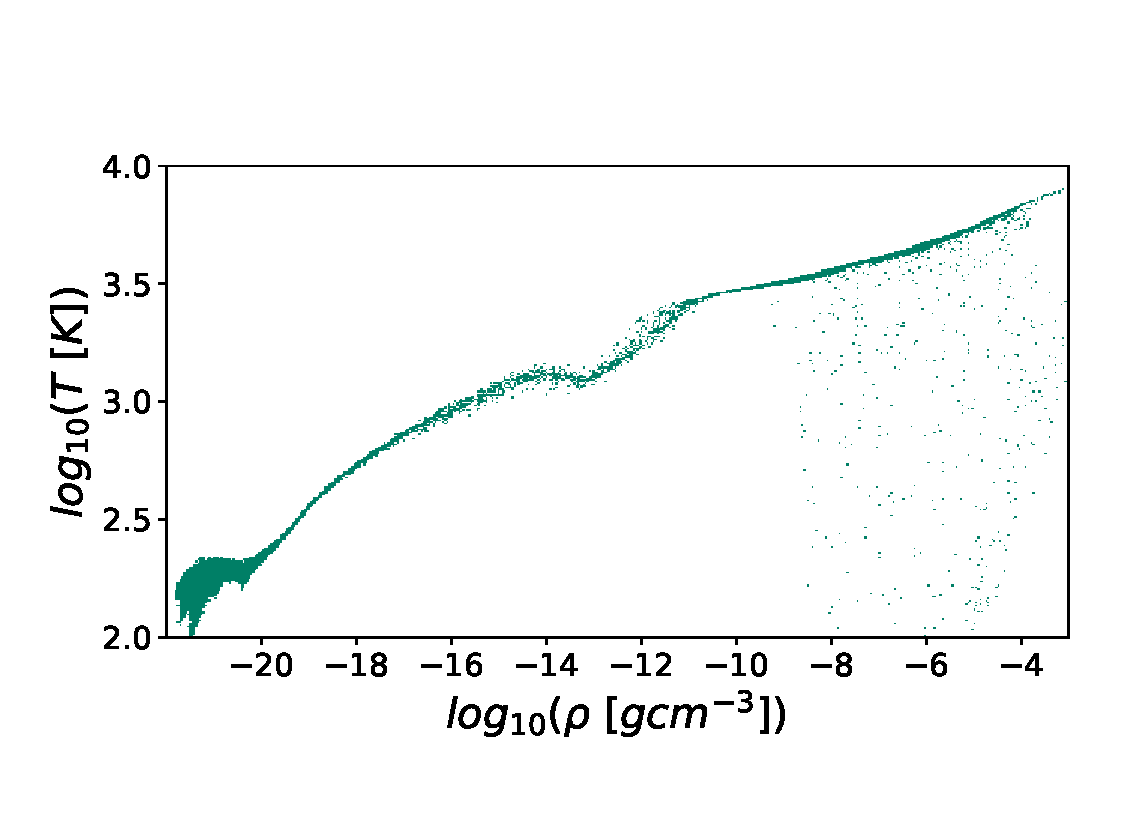
\includegraphics[scale=0.5]{simple.pdf}}
    \caption{Relationship between density and temperature during a collapse in the absence of turbulence, resulting in a single central dense object. As the computing time required is greater for pure collapse set-ups, the Jeans length was allowed to fall below the minimum cell size at at the highest densities, producing the artificial behaviour seen in the bottom right section of the figure.}
    \label{fig:simple}
\end{figure}

\begin{table}
	\centering
	\caption{Sink creation density, temperature, sink radius, minimum cell size and minimum gravitational softening lengths used in the study.}
	\label{table:1}
	\begin{tabular}{lcccr} % four columns, alignment for each
		\hline
		$\rho_{\text{sink}}$ [$gcm^{-3}$] & T [K] & $\lambda_J$ [cm] & $V_{\text{min}}$ [cm$^{3}$] & $L_{\text{soft}}$ [cm]\\
		\hline
		$10^{-10}$ & 3050 & 1.37$\times 10^{14}$ & 5.10$\times 10^{39}$ & 1.72$\times 10^{13}$\\
		$10^{-9}$ & 3350 & 4.56$\times 10^{13}$ & 1.86$\times 10^{38}$ & 5.70$\times 10^{12}$\\
		$10^{-8}$ & 3750 & 1.53$\times 10^{13}$ & 6.95$\times 10^{36}$ & 1.91$\times 10^{12}$\\
		$10^{-7}$ & 4100 & 5.05$\times 10^{12}$ & 2.51$\times 10^{35}$ & 6.31$\times 10^{11}$\\
		\hline
	\end{tabular}
\end{table}





\section{Simulations}
\label{Sims}
Four iterations were performed with identical initial conditions, with the moving mesh code AREPO \citep{Springel2010}. The sink parameters were varied as given in table \ref{table:1}. The chemistry used was the same as \cite{Clark2011}, with abundances of H$_2$, H$^{+}$, D$^{+}$ and HD as x$_{\text{H}_{2}}$=10$^{-3}$, x$_{\text{H}^{+}}$=10$^{-7}$, $x_{\text{D}^{+}}$=2.6$\times$10$^{-12}$ and $x_{\text{HD}}$=3$\times$10$^{-7}$. The initial conditions consist of a Bonner Ebert sphere, categorised by central density $n_c$=2$\times$10$^{-20}$ and radius R$_{\text{BE}}$=1.87pc. The sphere was placed in a box of side length 4R$_{\text{BE}}$. The density was enhanced by a factor of 1.87 to promote collapse and a random velocity field was imposed on the box, generated from the turbulent power spectrum $\propto k^{-2}$. The rms velocity was scaled to give a ratio of kinetic to gravitation energy $\alpha$=0.05 and the initial box temperature was 200K. The simulations were performed with refinement criteria of 16 cells per Jeans length. The evolution of N$_{\text{sink}}$ and M$_{\text{total}}$ is shown in figure \ref{fig:sinks_nomerge}.

\subsection{Sink mergers}
\cite{Bonnell2005} showed that massive stars can form through the merger of a high-mass close binary. The total number of sinks and their masses  would be unrepresentative of the IMF if they were allowed to bunch up and lie on top of one another without merging. The  simulations described in \ref{Sims} were repeated with sink mergers enabled, to produce a more reliable IMF. Similarly to \cite{Federrath2010}, we allow sinks to merge if they fit four criteria: they lie within eachothers accretion radius, they are moving towards eachother $(\nabla \cdot v) < 0$, their accelerations give $(\nabla \cdot a) <0$ and they are gravitationally bound. Since sink particles carry no thermal data, the last criteria simply requires that their gravitational potential well exceeds the kinetic energy of the system. When the criteria are met, the larger of the sinks gains the mass and linear momentum of smaller sink, and its position is shifted to the center of mass of the system. We allow multiple mergers per time-step, based on mass hierarchy; if sink A is flagged to merge into sink B, and sink B is flagged to merge into sink C, then both A and B will be merged into sink C simultaneously. The evolution of N$_{\text{sink}}$ and M$_{\text{total}}$ with sink mergers enabled is shown in figure \ref{fig:sinks}. The resulting clusters are shown at different stages of collapse in figure \ref{fig:grid}. The total number of sinks formed, total mass in sinks, largest sink mass, number of sinks ejected from the system and number of mergers are given in table \ref{table:2}, at 400 and 1200yrs after the formation of the first sink.

% Example figure
\begin{figure}
	% To include a figure from a file named example.*
	% Allowable file formats are eps or ps if compiling using latex
	% or pdf, png, jpg if compiling using pdflatex
	\hbox{\hspace{-0.8cm} 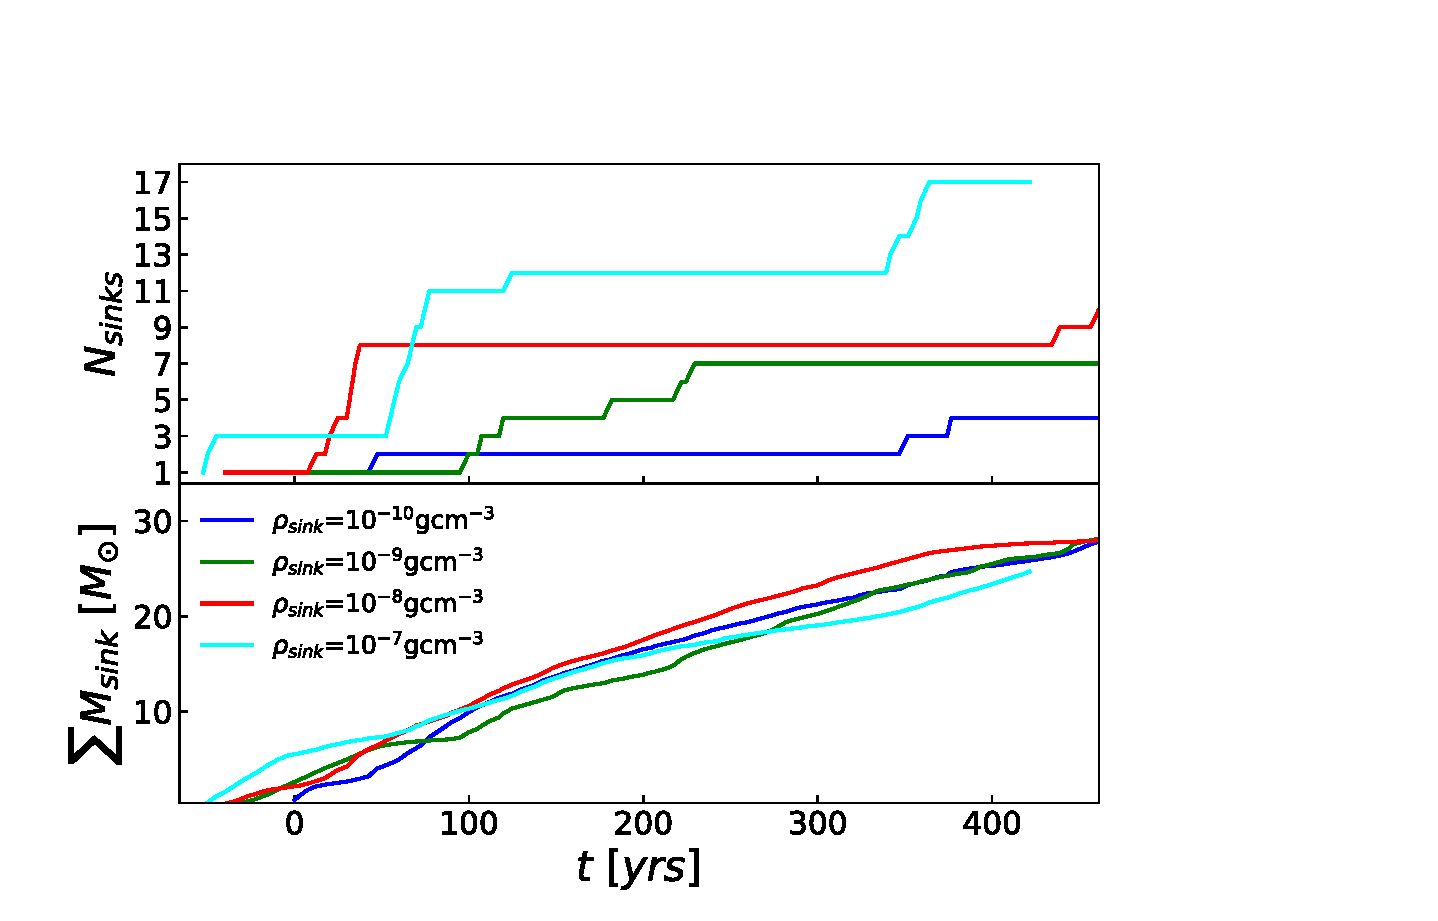
\includegraphics[scale=0.5]{sinks_nomergers.pdf}}
    \caption{Evolution of the number of sinks and the total mass of all sinks without sink mergers enabled.}
    \label{fig:sinks_nomerge}
\end{figure}

% Example figure
\begin{figure}
	% To include a figure from a file named example.*
	% Allowable file formats are eps or ps if compiling using latex
	% or pdf, png, jpg if compiling using pdflatex
	\hbox{\hspace{-0.9cm} 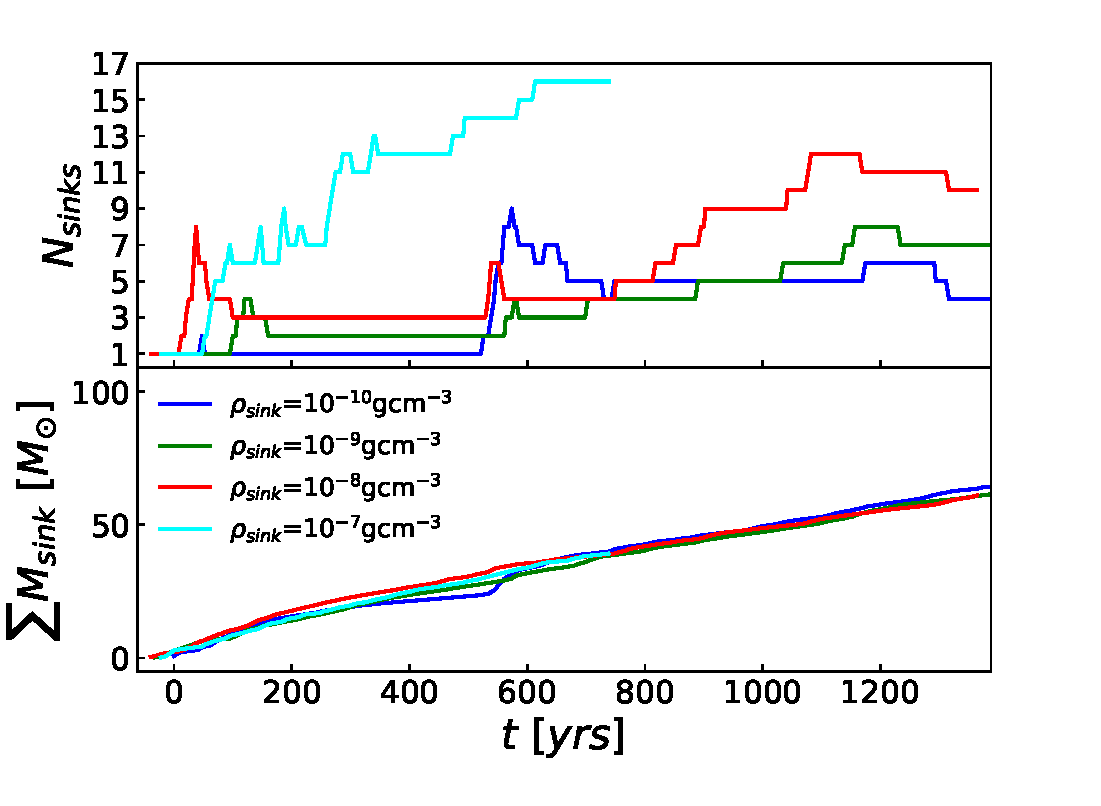
\includegraphics[scale=0.54]{sink_mergers.pdf}}
    \caption{Evolution of the number of sinks and the total mass of all sinks with sink mergers enabled.}
    \label{fig:sinks}
\end{figure}

% Example figure
\begin{figure*}
	% To include a figure from a file named example.*
	% Allowable file formats are eps or ps if compiling using latex
	% or pdf, png, jpg if compiling using pdflatex
	\hbox{\hspace{-2cm} 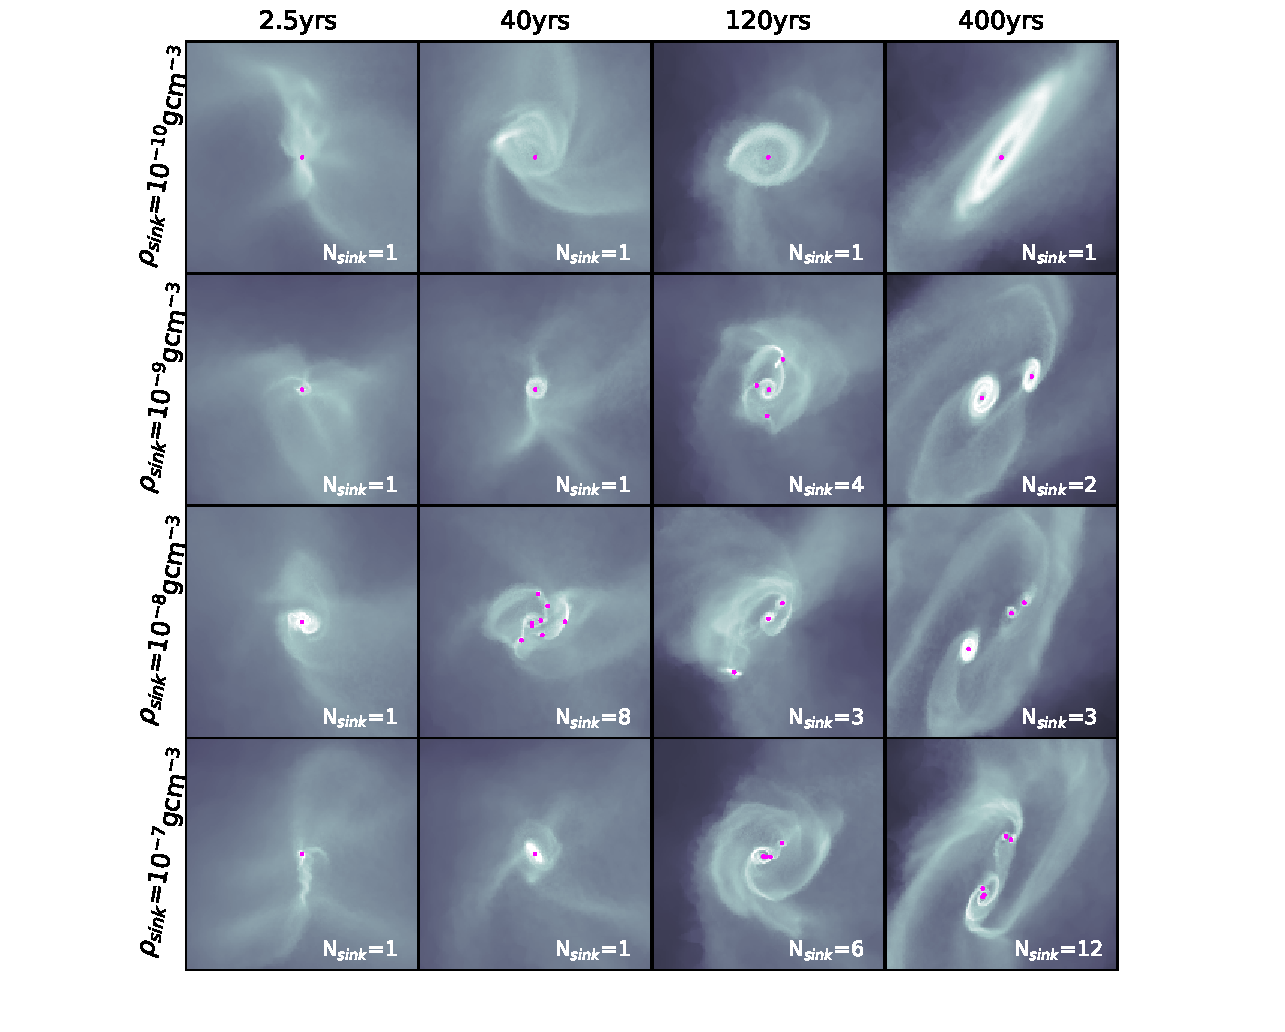
\includegraphics[scale=1]{grid1.pdf}}
    \caption{Density plots taken at 2.5, 40, 120 and 400 years after the formation of the first sink particle. A, B, C and D correspond to $\rho_{\text{sink}}$=$10^{-10}$,$10^{-9}$, $10^{-8}$ and $10^{-7}$. Sink particles are shown as red dots. The box lengths shown are all of side length 107AU. The simulations were performed with sink mergers enabled.}
    \label{fig:grid}
\end{figure*}



\begin{table*}
	\centering
	\caption{The total number of sinks formed, total mass in sinks, largest sink mass, number of sinks ejected from the system and number of mergers at 400 and 1200yrs after the formation of the first sink.}
	\label{table:2}
	\begin{tabular}{l c c c c c c c c c c c c c c c r } % four columns, alignment for each
		\hline
		& & & & & &  t=400yrs & & &  & & & & & t=1200yrs & \\
		\hline
		$\rho_{\text{sink}}$  & & & & N$_{\text{sink}}$ & M$_{\text{tot}}$ [M$_{\odot}$] & M$_{\text{largest}}$ [M$_{\odot}$] & N$_{\text{eject}}$ & N$_{\text{merge}}$ & & & & N$_{\text{sink}}$ & M$_{\text{tot}}$ [M$_{\odot}$] & M$_{\text{largest}}$ [M$_{\odot}$]  & N$_{\text{eject}}$ & N$_{\text{merge}}$ \\
		\hline
		$10^{-10}$  & & & & 1  & 21.33 &  21.33   & 0 &  1   & & &  & 6  &  57.43 &  29.20   &  0  &  7 \\
		$10^{-9}$   & & & &  2 & 23.63 &  14.39  & 0 & 2   & & & &  8  &  55.59 &    20.88   &0  &  3 \\
		$10^{-8}$    & & & &  3 & 26.59 &   9.09  & 0 & 5   & & & &  11 &  55.28 &    16.28   &3  &  9  \\
		$10^{-7}$  &  & & & 12 & 25.39 &   6.73  & 5 & 10 & & &  & -  &  -         &     -    & -  &  - \\
		\hline
	\end{tabular}
\end{table*}


% Example figure
\begin{figure}
	% To include a figure from a file named example.*
	% Allowable file formats are eps or ps if compiling using latex
	% or pdf, png, jpg if compiling using pdflatex
	 \hbox{\hspace{-0.5cm} 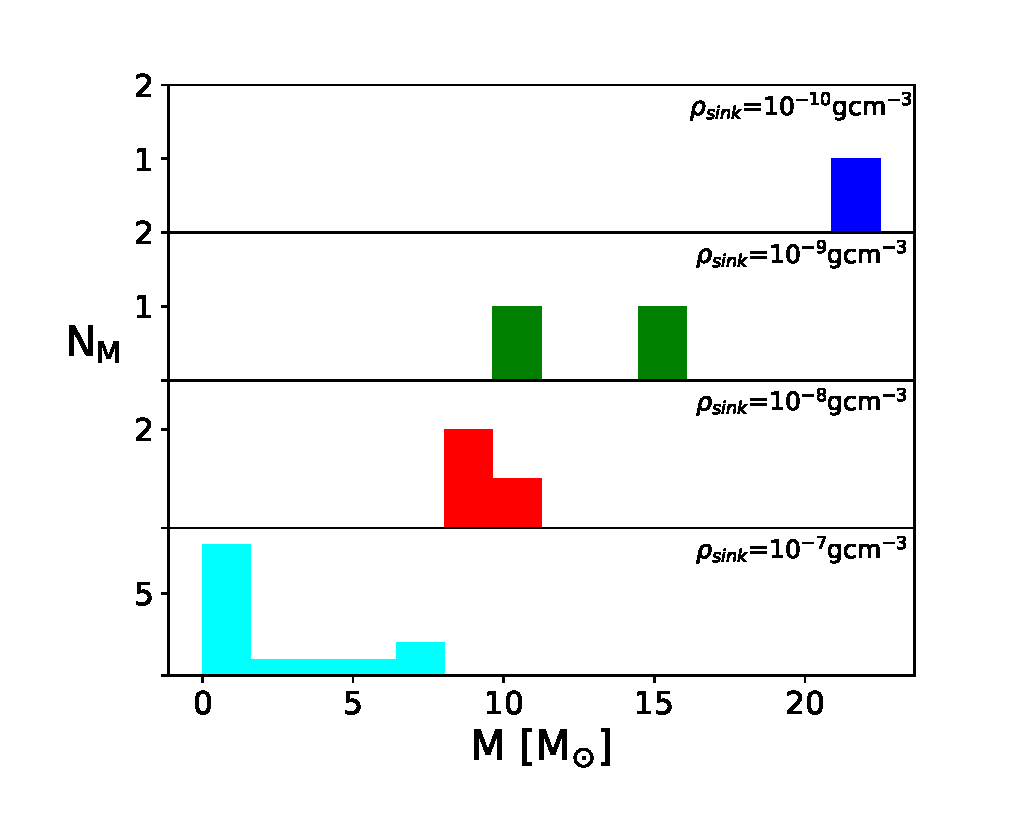
\includegraphics[scale=0.5]{IMF1.pdf}}
    \caption{Initial mass functions taken at $t\sim$500 years after the formation of the first sink. The distribution of masses shifts towards lower masses with increasing $\rho_{\text{sink}}$.}
    \label{fig:IMF}
\end{figure}
 
\section{Velocity power spectra}
To investigate possible effects of sink creation density on the resulting velocity field, we calculate the velocity power spectrum at the same time for each of the runs, at a time just after all of the runs have finished forming their first sink. The AREPO unstructured mesh of the inner $\sim$ 270AU region was projected onto a uniform $1000^3$ grid cube. Taking the Fourier transform of the velocity fields $A_v$ gives a 3-dimensional $k$ space of velocity amplitudes, where $k$ is the number of wavelengths per box length. The average energy in each $k$ mode $\hat A_v$ was found by averaging the amplitudes within $k$ shells, spanning out from $k$=1 to $k$=500 i.e the Nyquist frequency of the data. These $k$ modes correspond to physical scales of 270 to 0.5AU, the latter being roughly $\lambda_J$ of the highest resolution run. The power spectrum $P_v$ was obtained using

\begin{equation}
P_v \delta k = \int_{1}^{500} \hat A_v^2 4\pi k^2 \delta k 
\end{equation}

The radial velocity profile was removed before taking the Fourier transform, by taking the cross product $v_\theta=(v \times r)/|r|$, subtracting the effects of material falling into the sink, leaving the pure turbulent field. The resulting velocity power spectra are given in figure \ref{fig:spectrum}.

% Example figure
\begin{figure}
	% To include a figure from a file named example.*
	% Allowable file formats are eps or ps if compiling using latex
	% or pdf, png, jpg if compiling using pdflatex
	 \hbox{\hspace{-0.5cm} 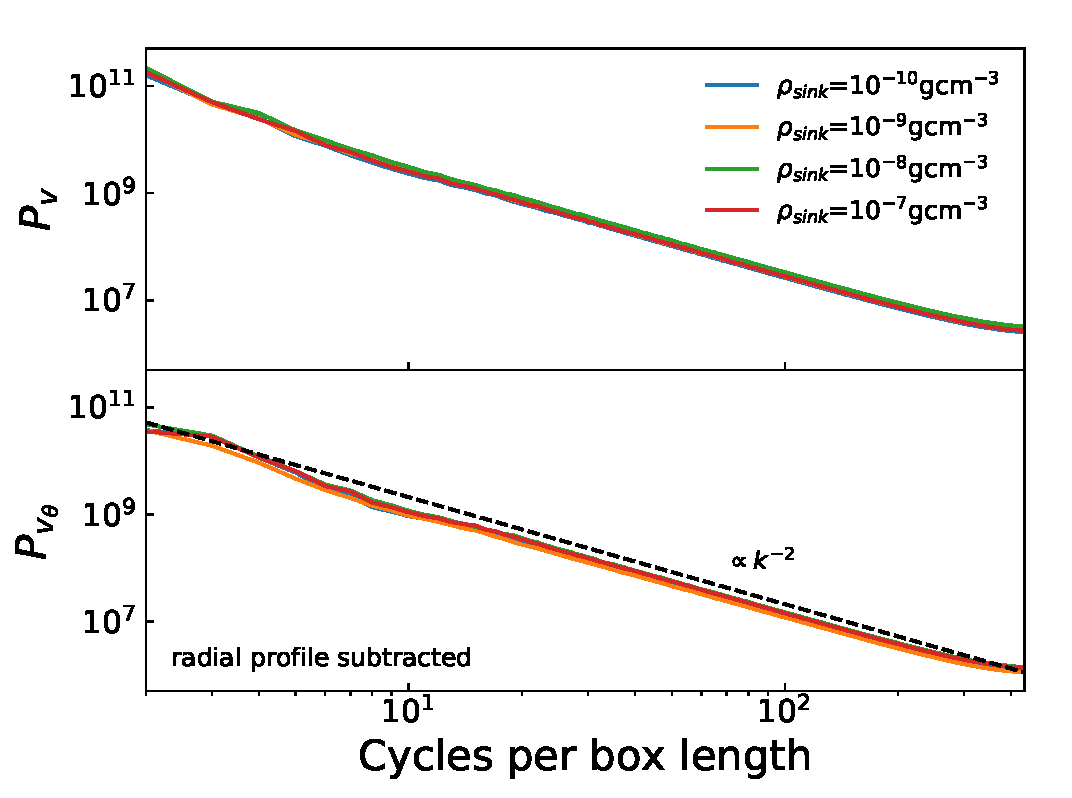
\includegraphics[scale=0.5]{velocity_spectrum.pdf}}
    \caption{The velocity power spectrum at $\sim$ 2.5yrs after the formation of the first sink. The velocity spectrum is independent of the chocie of N$_{\text{sink}}$.}
    \label{fig:spectrum}
\end{figure}



\section{Discussion}
Figure \ref{fig:sinks} shows that even with sink mergers enabled, the total number of sinks formed did not converge within the range of sink formation densities used. Higher values of $\rho_{\text{sink}}$ gave higher number of sinks formed. The number of sinks formed, total mass in sinks, highest mass sink, number of ejected sinks, and number of sink mergers are given in table \ref{table:2}, at t=400yrs and t=1200yrs after the formation of the first sink. N$_{\text{sink}}$ may converge for higher $\rho_{\text{sink}}$ than tested in this study, but it is currently computationally impractical to run collapse problems to densities that high if the study attempts to cover a large parameter space such as turbulent energy or magnetic field strength. For the first $\sim$500yrs, the total mass in sinks also increased with increasing $\rho_{\text{sink}}$. However, after 600yrs, the total mass in sinks became invariant with changing sink parameters. As higher $\rho_{\text{sink}}$ produces higher N$_{\text{sink}}$ while M$_{\text{tot}}$ remains unaffected, using higher $\rho_{\text{sink}}$ produces lower mass stars and a broadened IMF. The mass of the largest sink in the group also decreased with increasing resolution. The resulting IMFs at time $t\sim$ 500yrs are given in figure \ref{fig:IMF}, the distribution of stars shifts towards lower mass populations with increasing $\rho_{\text{sink}}$. For the lowest resolution run, a single dense object forms in agreement with early numerical Pop III work (\citealt{Bromm1999}, \citealt{Haiman1996}), however it fragments into a broader IMF after $\sim$600yrs. Generally, the number of mergers increased with increasing resolution. The number of ejections from the group also increased with resolution. Due to the sink accretion radius decreasing with increasing $\rho_{\text{sink}}$, sinks had to be closer together before they could merge for higher $\rho_{\text{sink}}$ runs, possibly preventing mergers that could have kept the sinks from being ejected. The lower resolution rows of figure \ref{fig:grid} show the formation of disks and subsequent fragmentation in the early stages of collapse, that are absent in higher resolution runs. Unresolved, turbulent motions can produce artificial, large scale rotation \citep{Seifried2017}, to which these disks may be attributed. Figure \ref{fig:spectrum} shows that the velocity power spectra after the formation of the first sink was also invariant with changing $\rho_{\text{sink}}$. The results show that numerically obtained IMFs using sink particles are reliant on the authors choice of $\rho_{\text{sink}}$, with higher resolution runs being more susceptible to fragmentation and less likely to merge under the current merger criteria. 


\section{Conclusions}

In a Population III setting, the number of sinks formed is reliant on the sink creation density. Higher sink creation densities result in larger number of sinks formed without converging within the range tested. The total mass in sinks is was independent of the sink parameters used after $\sim$600yrs, resulting in an IMF that shifts towards lower mass stars with higher sink creation density. The number of sink mergers and ejections from the system increased with increasing sink creation density. The velocity power spectra taken just after the formation of the first sinks reveal that varying the sink parameters do not affect the turbulent velocity field.

\section*{Acknowledgements}



%%%%%%%%%%%%%%%%%%%%%%%%%%%%%%%%%%%%%%%%%%%%%%%%%%


 





%%%%%%%%%%%%%%%%%%%% REFERENCES %%%%%%%%%%%%%%%%%%

% The best way to enter references is to use BibTeX:

\bibliographystyle{mnras}

\bibliography{references.bib} % if your bibtex file is called example.bib



%%%%%%%%%%%%%%%%%%%%%%%%%%%%%%%%%%%%%%%%%%%%%%%%%%

%%%%%%%%%%%%%%%%% APPENDICES %%%%%%%%%%%%%%%%%%%%%




%%%%%%%%%%%%%%%%%%%%%%%%%%%%%%%%%%%%%%%%%%%%%%%%%%


% Don't change these lines
\bsp	% typesetting comment
\label{lastpage}

\end{document}

% End of mnras_template.tex